\documentclass[utf8]{beamer}

\usepackage[T1]{fontenc}
\usepackage[brazil]{babel}
\usepackage{inconsolata}
\usepackage{minted}
\usepackage{tabu}
\usepackage[absolute, overlay]{textpos}
\usepackage{graphicx}
\usepackage{changepage} % adjustwidth environment

\definecolor{codebgcolor}{HTML}{FFFFFF}
\definecolor{coderulecolor}{HTML}{5F7FFF}
\definecolor{outerbgcolor}{HTML}{F0F0FF}

\setminted{autogobble,
           breaklines, breakanywhere,
           breaksymbolindentleft=0pt, breaksymbolindentright=0pt,
           breaksymbolsepleft=3pt, breaksymbolsepright=3pt,
           breaksymbolright=...,
           bgcolor=codebgcolor, style=paraiso-light,
           fontsize=\fontsize{10pt}{10pt},
           frame=lines, rulecolor=coderulecolor, framerule=.7pt}
\setmintedinline{bgcolor={}}

\mode<presentation>
\usetheme{Warsaw}
\setbeamercolor{structure}{fg=red!20!black}
\setbeamercolor{background canvas}{bg=outerbgcolor}
\beamertemplatenavigationsymbolsempty

\setbeamertemplate{footline}{\leavevmode\hbox{%
  \begin{beamercolorbox}[wd=.35\paperwidth, ht=2.25ex, dp=1ex, center]
                        {author in head/foot}
    \usebeamerfont{author in head/foot}
      Danilo J. S. Bellini \hfill \texttt{@danilobellini}
  \end{beamercolorbox}%
  \begin{beamercolorbox}[wd=.65\paperwidth, ht=2.25ex, dp=1ex, center]
                        {title in head/foot}
    \usebeamerfont{title in head/foot}
      \insertshorttitle \hfill
      CryptoRave -- SP \hfill
      \insertshortdate \hfill
      \insertframenumber\,/\,\inserttotalframenumber
  \end{beamercolorbox}%
}}

\title{Tomb}
\subtitle{Do GPG à esteganografia na prática}
\author{Danilo J. S. Bellini \\ \texttt{@danilobellini}}
\date{2019-05-04}

\setlength{\TPHorizModule}{\paperheight}
\setlength{\TPVertModule}{\paperheight}

\renewcommand{\thefootnote}{[\arabic{footnote}]}

\newcommand{\includesvg}[2]{%
  \ifnum\pdfstrcmp{\pdffilemoddate{#2.svg}}%
                  {\pdffilemoddate{#2.pdf}}>0%
    {\immediate\write18%
     {inkscape -z -D --file=#2.svg --export-pdf=#2.pdf --export-latex}%
    }%
  \fi%
  \centering%
  \resizebox{#1}{!}{%
    \input{#2.pdf_tex}%
  }%
}


\begin{document}


\begin{frame}
  \titlepage
  \center
    {\Huge CryptoRave} \\ \vfill
    Biblioteca Mário de Andrade, São Paulo -- SP
  \begin{textblock}{0}(.05, .52)%
    \includegraphics[height=50pt]{cr_logo.png}%
  \end{textblock}
  \begin{textblock}{0}(.93, .47)%
    
\includegraphics[height=80pt]{tomb_n_bats.png}%
  \end{textblock}
\end{frame}


\begin{frame}{Criptografia}
  Criptografia é a prática e o estudo
  das técnicas de armazenamento e comunicação de informação
  na presença de terceiros/adversários.
  Os usos da criptografia estão relacionados a
  diferentes aspectos da segurança da informação (\emph{security}):
  \vfill
  \begin{itemize}
    \item
    Integridade:
    \textbf{Assinatura} (\emph{Sign})
    \item
    Confidencialidade / Privacidade: \\
    \textbf{Encriptação/decriptação} (\emph{Encrypt/Decrypt})
  \end{itemize}
  \vfill
  Classificamos os algoritmos de acordo com o número de chaves:
  \vfill
  \begin{itemize}
    \item Criptografia de chave simétrica \\
          (chave única, de conhecimento exclusivo das partes)
    \item Criptografia de chave pública \\
          (pares de chave pública/privada para cada parte)
    \item Funções de \emph{hash} (sem chave)
  \end{itemize}
  \begin{textblock}{0}(1, .01)%
    \includesvg{70pt}{Crypto_key}%
  \end{textblock}
\end{frame}


\begin{frame}[fragile]{Chave simétrica:
                       Cifras de César, Vigenère e autochave}
  \begin{columns}[c]
    \column{.55\textwidth}
    \resizebox{\textwidth}{!}{%
      \begin{tabular}{rl} \textbf{Cifra de César} \\
                Chave: & \texttt{C} \hfill
                         \emph{\tiny(Desloca 2 no alfabeto,
                                     A \textrightarrow C)} \\
        Chave efetiva: & \texttt{CC CCCCC CC CCCCCCCC} \\ \hline
             Mensagem: & \texttt{EU GOSTO DE LIMONADA} \\
        Texto cifrado: & \texttt{GW IQUVQ FG NKOQPCFC} \\
      \end{tabular}%
    }
    \vspace{.5em}\vfill
    A cifra de César transforma cada caractere da mensagem
    usando uma tabela como esta:
    \vspace{1em}\vfill
    \resizebox{\textwidth}{!}{%
      \begin{tabular}{c|c|c|c}
        \texttt{A} \textrightarrow \texttt{C} &
        \texttt{B} \textrightarrow \texttt{D} &
        \texttt{C} \textrightarrow \texttt{E} &
        \texttt{D} \textrightarrow \texttt{F} \\
        \texttt{E} \textrightarrow \texttt{G} &
        \texttt{F} \textrightarrow \texttt{H} &
        \texttt{G} \textrightarrow \texttt{I} &
        \texttt{H} \textrightarrow \texttt{J} \\
        \texttt{I} \textrightarrow \texttt{K} &
        \texttt{J} \textrightarrow \texttt{L} &
        \texttt{K} \textrightarrow \texttt{M} &
        \texttt{L} \textrightarrow \texttt{N} \\
        \texttt{M} \textrightarrow \texttt{O} &
        \texttt{N} \textrightarrow \texttt{P} &
        \texttt{O} \textrightarrow \texttt{Q} &
        \texttt{P} \textrightarrow \texttt{R} \\
        \texttt{Q} \textrightarrow \texttt{S} &
        \texttt{R} \textrightarrow \texttt{T} &
        \texttt{S} \textrightarrow \texttt{U} &
        \texttt{T} \textrightarrow \texttt{V} \\
        \texttt{U} \textrightarrow \texttt{W} &
        \texttt{V} \textrightarrow \texttt{X} &
        \texttt{W} \textrightarrow \texttt{Y} &
        \texttt{X} \textrightarrow \texttt{Z} \\
        \texttt{Y} \textrightarrow \texttt{A} &
        \texttt{Z} \textrightarrow \texttt{B}
      \end{tabular}%
    }

    \column{.55\textwidth}
    \resizebox{\textwidth}{!}{%
      \begin{tabular}{rl} \textbf{Cifra de Vigenère} \\
                Chave: & \texttt{MENTIRA} \\
        Chave efetiva: & \texttt{ME NTIRA ME NTIRAMEN} \\ \hline
             Mensagem: & \texttt{EU GOSTO DE LIMONADA} \\
        Texto cifrado: & \texttt{QY THAKO PI YBUFNMHN} \\ \hline \hline
                Chave: & \texttt{PAGAZAQ} \\
        Chave efetiva: & \texttt{PA GAZAQ PA GAZAQPAG} \\ \hline
             Mensagem: & \texttt{EU GOSTO DE LIMONADA} \\
        Texto cifrado: & \texttt{TU MORTE SE RILODPDG} \\
      \end{tabular}
    }
    \vspace{.5em}\vfill
    Generalizações: um deslocamento diferente para cada caractere,
    ou ``circular'' ou com a própria mensagem continuando a chave.
    \vspace{1em}\vfill
    \resizebox{\textwidth}{!}{%
      \begin{tabular}{rl} \textbf{Autochave} \\
                Chave: & \texttt{PAGAZAQP} \\
        Chave efetiva: & \texttt{PA GAZAQ PE UGOSTODE} \\ \hline
             Mensagem: & \texttt{EU GOSTO DE LIMONADA} \\
        Texto cifrado: & \texttt{TU MORTE SI FOAGGOGE} \\
      \end{tabular}%
    }
  \end{columns}
\end{frame}


\begin{frame}[fragile]{GPG~-- \emph{GNU Privacy Guard}}
  O GPG é uma implementação em software livre (GPLv3)
  que atende ao OpenPGP\footnote{
      PGP significa \emph{Pretty Good Privacy},
      um software comercial criado em 1991.
      Sua segunda versão formou o [hoje obsoleto] padrão RFC1991.
      A menos de uma atualização relativa ao algoritmo Camellia,
      RFC4880 (OpenPGP) é a versão mais recente do padrão.
    }
  sem utilizar softwares/algoritmos patenteados/restritos/privados.
  \vfill
  Vamos utilizá-lo para criptografia de chave simétrica!
  \vfill
  \begin{minted}{shell}
    echo CryptoRave > m.txt    # Criando uma mensagem
    gpg -c -o m.txt.gpg m.txt  # Encriptação! GPG pede senha 2x
    hexdump -C m.txt.gpg       # O resultado é binário...
    file m.txt.gpg             # ... com metadados abertos

    # Em outra máquina, ou depois de um killall gpg-agent
    # (pois o gpg lembra sua senha por um certo tempo)
    gpg -d m.txt.gpg m_decrypted.txt     # Decriptação!
  \end{minted}
\end{frame}


\begin{frame}[fragile]{GPG: \texttt{-c}/\texttt{--symmetric},
                            \texttt{-o}/\texttt{--output} e
                            \texttt{-d}/\texttt{--decrypt}}
  \begin{minted}{shell}
    seq 5 > mensagem.txt   # Outra mensagem: sequência de 1 a 5

    # Encriptação! Há muitas formas de fazer a mesma coisa
    gpg --symmetric --output mensagem1.txt.gpg mensagem.txt
    gpg -c -o mensagem2.txt.gpg mensagem.txt

    # Também podemos usar standard streams
    gpg -c --output mensagem4.txt.gpg < mensagem.txt
    gpg -c < mensagem.txt > mensagem4.txt.gpg

    # Mas chamadas consecutivas do mesmo comando,
    # mesmo com a mesma entrada, não devolvem o mesmo resultado!
    ls mensagem?.txt.gpg | xargs -n1 hexdump -C

    # Algo similar vale com a decriptação!
    gpg --decrypt -o mensagem1_decrypted.txt mensagem1.txt.gpg
    gpg -d mensagem2.txt.gpg > mensagem2_decrypted.txt
  \end{minted}
\end{frame}


\begin{frame}{Chave pública/privada}
  \begin{adjustwidth}{2em}{1em}\emph{\Huge
    ``Envio pelo correio um cadeado aberto sem a chave,
    o destinatário recebe,
    tranca um pacote com o cadeado e envia p/ mim.''
  }\end{adjustwidth}
  \vfill
  \begin{center}
    \begin{tabular}{rcl}
      Cadeado & \textrightarrow & Chave pública \\
      Chave do cadeado & \textrightarrow & Chave privada \\
    \end{tabular}
  \end{center}
\end{frame}


\begin{frame}[fragile]{Diffie-Hellman:
                       Algoritmo para troca de chave}
  \begin{columns}[c]
    \column{.5\textwidth}
    \vspace*{-1em}
    \begin{center}
      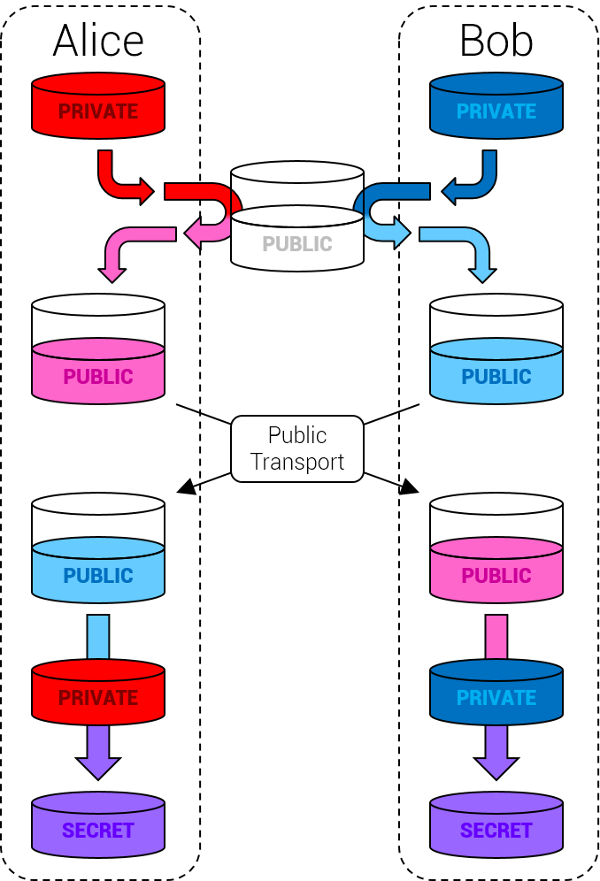
\includegraphics[height=.85\textheight]{diffie-hellman-paint.png}
      \fontsize{8pt}{8pt}\selectfont
      Imagem obtida em
      \url{http://crypto.mdc.io/2012/10/13/public-key-cryptography/}
    \end{center}
    \column{.6\textwidth}
    \resizebox{\textwidth}{!}{%
      \begin{tabular}{rl}
        Número primo (público): & $p$ \\
        Base (público): & $g$ \\
        Chave privada da Alice: & $a$ \\
        Chave pública da Alice: & $A = g^a \mod p$ \\
        Chave privada do Bob: & $b$ \\
        Chave pública do Bob: & $B = g^b \mod p$ \\
        Número compartilhado: & $A^b \equiv B^a \mod p$
      \end{tabular}%
    }
    \vspace{.5em}\vfill
    Exemplo (\emph{bash}):
    \begin{minted}{shell}
      # Alice e Bob combinam os parâmetros
          p=2551  ;  g=2
      # Criam chaves privadas em silêncio
          a=45    ;  b=29
      # Calculam e trocam chaves públicas
          A=$[(g ** a) % p]       # 2285
          B=$[(g ** b) % p]       # 207
      # Alice e Bob possuem um segredo!
          secret_b=$[(A ** b) % p]   # 414
          secret_a=$[(B ** a) % p]   # 414
    \end{minted}
  \end{columns}
\end{frame}


\begin{frame}[fragile]{GPG: Chaves públicas e privadas}
  Vamos utilizar o GPG com criptografia de chave pública!
  Primeiro, precisamos ter um par de chaves,
  p/ trocarmos as chaves públicas.
  \vfill
  \begin{minted}{shell}
    gpg --gen-key # Cria chaves (par público/privado)
    gpg -k        # Lista key IDs de chaves disponíveis (todas)
    gpg --list-keys                           # Idem    (todas)
    gpg --list-secret-keys                    # Idem (privadas)

    # Exportando/importando chaves públicas (com "--armor/-a")
    gpg --export --armor email@example.br > mykey.asc
    gpg --import mykey.asc

    # Também é possível exportar em formato binário (sem "-a")
    gpg --export email@example.br > mykey.gpg

    # E converter o formato depois de exportar
    gpg --enarmor binkey  # binkey.asc a partir do binkey
    gpg --dearmor asckey  # asckey.gpg a partir do asckey

    # Alternativa ao envio do arquivo: servidores de keyIDs
    gpg --keyserver pgp.mit.edu --send-keys keyID  # Envio
    gpg --keyserver pgp.mit.edu --recv-keys keyID  # Recebimento
  \end{minted}
\end{frame}


\begin{frame}[fragile]{GPG: \texttt{-b}/\texttt{--detach-sign},
                            \texttt{--verify} e
                            \texttt{-e}/\texttt{--encrypt}}
  Temos nosso par de chaves (pública e privada),
  e as partes envolvidas já importaram as chaves públicas
  dos demais. E agora?
  \vfill
  \begin{minted}{shell}
    # Assinatura em arquivo à parte (--detach-sign)
    gpg -u email@example.br -b m.txt  # Assina cria m.txt.sig
    gpg --verify m.txt.sig m.txt      # Verifica a assinatura

    # Encriptando (--encrypt) c/ a chave pública do destinatário
    gpg -o encrypted.gpg -r destino@example.br -e message.txt

    # Decriptando (--decrypt) com a chave privada
    gpg -o decrypted.txt -d encrypted.gpg
  \end{minted}
  \vfill
  O \mintinline{shell}{-u/--local-user}
  define qual é a chave privada que assina,
  e o GPG trabalha com uma chave privada padrão
  quando esse parâmetro não é fornecido.
  \vfill
  O \mintinline{shell}{-r/--recipient} é o destinatário.
  O \mintinline{shell}{-R/--hidden-recipient} funciona da mesma forma,
  mas não informa qual é o key ID do destinatário
  nos metadados do resultado.
\end{frame}


\begin{frame}[fragile]{\emph{Loopback device mount}}
  Discos rígidos, SSDs, SDs e outras mídias
  nem sempre estão criptografados,
  e às vezes gostaríamos de ver um diretório criptografado,
  sem nos preocuparmos com os outros diretórios.
  \vfill
  Como fazer um diretório (ou ponto de montagem)
  ser o acesso ao conteúdo de um arquivo de armazenamento?
  \vfill
  \begin{minted}{shell}
    # Cria a imagem "virtual.volume" vazia com 30MB
    dd if=/dev/zero of=virtual.volume bs=1M count=30
    # Formata o arquivo "virtual.volume" como ext4
    mkfs.ext4 virtual.volume
    # Criamos o diretório para ser o ponto de montagem
    sudo mkdir /mnt/virtual
    # Comandos para montar e desmontar o volume virtual
    sudo mount -o loop virtual.volume /mnt/virtual
    sudo umount /mnt/virtual
  \end{minted}
  \vfill
  Essas últimas operações precisam ser feitas com \texttt{sudo},
  mas há formas de contornar essa necessidade,
  por exemplo:
  \vfill
  \begin{center}
    \mintinline{shell}{udisksctl loop-setup -f virtual.volume}
  \end{center}
\end{frame}


\begin{frame}[fragile]{Tomb: armazenamento criptografado em um arquivo}
  \emph{Tomb} é uma ferramenta de criação e utilização
  de arquivos encriptados de armazenamento.
  A criptografia do ponto de montagem é feita
  por meio de uma chave específica do Tomb,
  separada do repositório de chaves do GPG,
  mas essa própria chave do Tomb é encriptada usando o GPG.
  \vfill
  \begin{minted}{shell}
    # Criação do arquivo para ser a imagem (com e sem o tomb)
    tomb dig new.tomb -s 50          # Cria o new.tomb com 50MB
    dd if=/dev/urandom of=new.tomb bs=1M count=50        # Idem

    # Criação de um arquivo de chave do tomb, encriptado com...
    tomb forge new.key                # Senha (chave simétrica)
    tomb forge new.key -g -r email@example.br   # Chave pública

    # Inicializa, atribui a chave e formata (requer loop mount)
    # (Dica: a partir do -k são os mesmos parâmetros do forge)
    tomb lock new.tomb -k new.key -g -r email@example.br
  \end{minted}
  \textcolor{red}{\small
    Hoje, no Arch Linux,
    é preciso alterar o Tomb
    p/ incluir o \texttt{-{}-type luks1} descrito em
    \url{https://github.com/dyne/Tomb/issues/343} (\emph{bugfix}).
  }
\end{frame}


\begin{frame}[fragile]{Tomb: armazenamento criptografado em um arquivo}
  Criamos o armazenamento criptografado em um arquivo! Como usar?
  \vfill
  \begin{minted}{shell}
    # Monta o new "como se fosse um pendrive"
    tomb open new.tomb -k new.key -g

    # Desmonta o new
    tomb close new
  \end{minted}
  \vfill
  Como utilizamos chaves públicas GPG,
  podemos passar múltiplas chaves
  no momento da criação de outro arquivo como o \texttt{new.tomb}.
  Isso significa que um único ``tomb''
  pode ser compartilhado entre múltiplos usuários.
  \vfill
  Aviso: Infelizmente
  os comandos \texttt{open}, \texttt{close} e \texttt{lock}
  exigem que o usuário possa chamar o \texttt{mount -o loop}
  visto anteriormente, o que exige um superusuário.
\end{frame}


\begin{frame}[fragile]{Esteganografia}
  Esteganografia refere-se a ocultar uma informação dentro de outra.
  No nosso caso, ocultaremos em uma imagem a chave usada
  para acesso ao Tomb (usando Steghide\footnote{
    \url{http://steghide.sourceforge.net/}
  }).
  \vfill
  \begin{minted}{shell}
    # Criemos uma imagem JPG (pode ser uma foto)
    convert cr_logo.png fakelogo.jpg

    # Armazena a chave na imagem, usando (mais uma) senha
    tomb bury fakelogo.jpg -k new.key -g

    # Para extrair a chave da imagem (sabendo a senha)
    tomb exhume fakelogo.jpg -k copy.key

    # Podemos usar a própria imagem como arquivo de chave
    tomb open new.tomb -k fakelogo.jpg -g
  \end{minted}
  \vfill
  A imagem processada é a do logo da CryptoRave.
  Não deverá haver diferença visual perceptível,
  e somente o portador da senha sabe que há uma chave nessa imagem.
\end{frame}


\begin{frame}[fragile]{Tomb: outros recursos}
  Entre os recursos adicionais que vale destacar,
  estão os \emph{hooks} que permitem a montagem automática
  de diferentes diretórios junto ao comando \texttt{tomb open}.
  Para isso, basta criar um arquivo no diretório raiz do ``tomb''
  chamado \texttt{bind-hooks}, com o conteúdo como:
  \begin{minted}{shell}
    caminho/dentro/do/tomb caminho/relativo/ao/home/do/usuario
    dados Desktop/Dados
  \end{minted}
  Para algo mais sofisticado,
  basta criar um script (com \emph{shebang})
  chamado \texttt{post-hooks}
  no diretório raiz do ``tomb''.
  Ele será executado automaticamente após o \texttt{tomb open}.
  \vfill
  Maiores informações sobre o Tomb podem ser encontradas em:
  \begin{itemize}
    \item \url{https://github.com/dyne/Tomb/wiki/Advancedfeatures}
    \item \url{https://wiki.archlinux.org/index.php/Tomb}
    \item \url{https://www.dyne.org/software/tomb/}
  \end{itemize}
\end{frame}


\begin{frame}
  \begin{center}\fontsize{5cm}{2.5cm}\selectfont
    FIM!
  \end{center}
\end{frame}


\end{document}
